\documentclass[journal]{IEEEtran}
\usepackage[a5paper, margin=10mm, onecolumn]{geometry}
\usepackage{lmodern, tfrupee, cite, amsmath, amssymb, amsfonts, amsthm, algorithmic, graphicx, textcomp, xcolor, txfonts, listings, enumitem, mathtools, gensymb, comment, hyperref, tkz-euclide, longtable, multicol, multirow, hhline, ifthen, lscape}

\begin{document}

\bibliographystyle{IEEEtran}
\vspace{3cm}

\title{11.16.1.11}
\author{EE24BTECH11008 - Aslin Garvasis}
\maketitle

\textbf{Question}:\newline
Suppose $3$ bulbs are selected at random from a lot. Each bulb is tested and classified as defective (D) or non-defective (N). Find the PMF of the random variable using the sum of three independent Bernoulli trials.\\ Take $P(N) = \frac{1}{2}.$

\textbf{Solution}:\newline
Let $X$ be a discrete random variable representing the number of non-defective bulbs from the three selected bulbs:
\begin{align}
    X = X_1+X_2+X_3
\end{align}
where $X_1, X_2, X_3 \sim \text{Bernoulli}(p=0.5)$. 

\begin{align}
    X_i = \begin{cases} 1, & \text{Non-defective} \\ 0, & \text{Defective} \end{cases}
\end{align}
Thus, $X \sim \text{Binomial}(n=3, p=0.5)$.

\textbf{Moment-Generating Function (MGF) Using the Z-Transform:}
\begin{align}
    M_{X_i}(z) &= (1-p) + p z^{-1}
\end{align}
Since $X_1, X_2, X_3$ are independent,
\begin{align}
    M_X(z) &= \big( (1-p) + p z^{-1} \big)^3 \\
           &= \sum_{n=0}^{3} \binom{3}{n} (1-p)^{3-n} p^n z^{-n}
\end{align}

Substituting $p=\frac{1}{2}$:
\begin{align}
    p_{X}(n) &= \frac{\binom{3}{n}}{8}, \quad n \in \{0,1,2,3\}
\end{align}

\textbf{Probability Mass Function (PMF):}
\begin{align}
    p_X(n) = \begin{cases} 
        \frac{1}{8}, & n = 0 \\
        \frac{3}{8}, & n = 1 \\
        \frac{3}{8}, & n = 2 \\
        \frac{1}{8}, & n = 3 
    \end{cases}
\end{align}

The graph below compares the theoretically calculated and simulated PMF of the given random variable.
\begin{figure}[htbp]
  \centering
  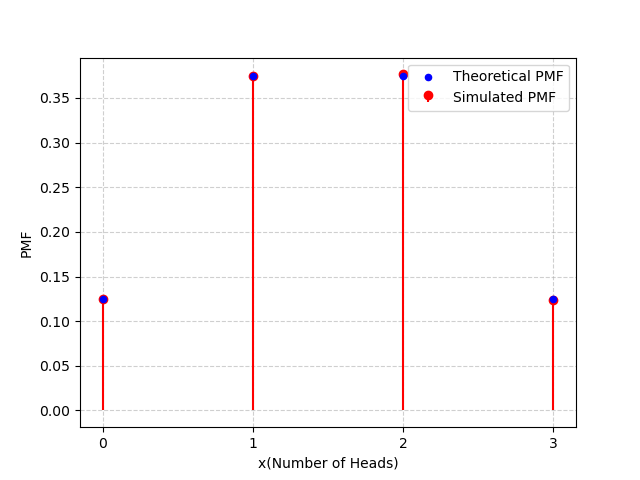
\includegraphics[width=\columnwidth]{figs/Fig1.png}
\end{figure}

\end{document}

